\documentclass{article}
\usepackage{fontspec}  % For custom font support (required by xelatex)
\usepackage[greek,english]{babel}
\setmainfont{Times New Roman}  % You can use any system-installed font

\usepackage{graphicx}
\usepackage{listings}
\usepackage{xcolor}

\lstdefinestyle{cppstyle}{
    language=C++,
    basicstyle=\ttfamily\footnotesize,
    keywordstyle=\color{blue},
    commentstyle=\color{gray},
    stringstyle=\color{teal},
    backgroundcolor=\color{white},
    frame=single,
    breaklines=true,
    breakatwhitespace=false,
    tabsize=4,
    showstringspaces=false,
    captionpos=b
}

\title{Simulating Branch Prediction with PIN}
\author{Χαράλαμπος Παπαδόπουλος \\03120199}
\date{Απρίλιος 2025}

\begin{document}

\maketitle

\section{Εισαγωγή}

Ζητούμενο της άσκησης είναι η κατασκευή και σε συνέχεια η σύγκριση διάφορων branch predictors χρησιμοποιώντας το εργαλείο προσομοίωσης PIN.

\section{Ανάλυση εντολών άλματος}
Αρχικά, συλλέγουμε δεδομένα σχετικά με τα benchmarks που θα χρησιμοποιήσουμε (τόσο για τα train όσο και για τα ref) χρησιμοποιώντας το pintool cslab\_branch\_stats.so. Λαμβάνουμε, λοιπόν τα εξής αποτελέσματα:

ΠΟΛΛΑ ΔΙΑΓΡΑΜΜΑΤΑ

\section{Ν-bit predictors}
Σε αυτό το ερώτημα πλέον ξεκινάμε την ανάλυση κάποιων branch predictors.
\subsection{}
 Διατηρώντας σταθερό τον αριθμό των BHT entries και ίσο με 16Κ, προσομοιώνουμε τους n-bit
predictors, για Ν = 1, 2, 3, 4. Τα n-bits υλοποιούν ένα saturating up-down counter (cslab\_branch.cpp) όπως είδαμε στις διαλέξεις.

Τροποιούμε κατάλληλα τον βοηθητικό κώδικα προσθέτοντας τον εξής κώδικα
\begin{lstlisting}[style=cppstyle]
   for (int i=1; i <= 4; i++) {
       NbitPredictor *nbitPred = new NbitPredictor(14, i);
       branch_predictors.push_back(nbitPred);
   }
\end{lstlisting}
Οι παράμετροι που δίνουμε στο object \texttt{NbitPredictor} είναι:
\begin{itemize}
    \item \texttt{index\_bits = 14}~: Ορίζει το πλήθος των bits που χρησιμοποιούνται για την κατασκευή του πίνακα προβλέψεων. Δηλαδή, το μέγεθος του πίνακα θα είναι $2^{14}$ καταχωρήσεις.
    \item \texttt{cntr\_bits}~: Ορίζει το πλήθος των bits κάθε μετρητή στον πίνακα. Όσο περισσότερα bits, τόσο περισσότερες καταστάσεις μπορεί να περιγράψει ένας μετρητής.

\end{itemize}
Καταλήγουμε, λοιπόν, με τα εξής διαγραμμάτα:

ΠΟΛΛΑ ΔΙΑΓΡΑΜΜΑΤΑ

ΣΥΜΠΕΡΑΣΜΑΤΑ

\subsection{}
Από το paper \textit{“Optimal 2-Bit Branch Predictors”} (R. Nair, 1995) βλέπουμε τα εξής πιθανά FSM:

\begin{figure}[h!]
    \centering
    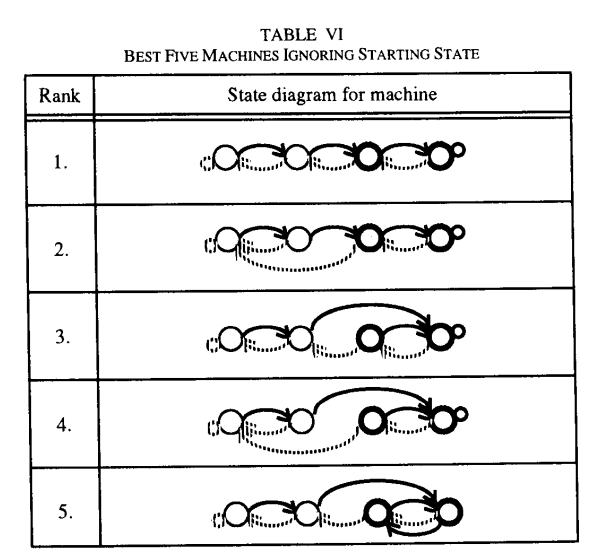
\includegraphics[width=0.5\linewidth]{figures/FMS.png}
    \caption{FSMs according to R. Nair.}
    \label{fig:enter-label}
\end{figure}

όπου με \textbf{bold} απεικονίζονται οι μεταβάσεις μετά από σωστή πρόβλεψη και \texttt{dotted} οι μεταβάσεις ύστερα από αποτυχημένη.

Βασιζόμενοι σε αυτά τα διαγράμματα δημιουργούμε τους αντίστοιχους predictors στο αρχείο branch\_predictor.h:
\begin{lstlisting}[style=cppstyle]
class TwobitPredictor_FSM2 : public BranchPredictor
{
public:
    TwobitPredictor_FSM2(unsigned index_bits_ = 14, unsigned cntr_bits_ = 2)
    \\same as before ...

    virtual void update(bool predicted, bool actual, ADDRINT ip, ADDRINT target) {
        unsigned int ip_table_index = ip % table_entries;
        if (actual) {
            if (TABLE[ip_table_index] < COUNTER_MAX)
                TABLE[ip_table_index]++;
        } else {
            if (TABLE[ip_table_index] == 2)
                TABLE[ip_table_index] -= 2;
            else if (TABLE[ip_table_index] > 0)
                TABLE[ip_table_index]--;
        }
        
        updateCounters(predicted, actual);
    };

    virtual string getName() {
        std::ostringstream stream;
        stream << "FSM2_" << pow(2.0,double(index_bits)) / 1024.0 << "K-" << cntr_bits;
        return stream.str();
    }
\end{lstlisting}
Κατά αντίστοιχο τρόπο κατασκευάζουμε και τις υπόλοιπες κλάσεις τις οποίες μετά καλούμε στο cslab\_branch.cpp

\begin{lstlisting}[style=cppstyle]
new TwobitPredictor_FSM1();
new TwobitPredictor_FSM2();
new TwobitPredictor_FSM3();
new TwobitPredictor_FSM4();
new TwobitPredictor_FSM5();
\end{lstlisting}

ΔΙΑΓΡΑΜΜΑΤΑ

ΣΥΜΠΕΡΑΣΜΑΤΑ

\subsection{}
Προκειμένου να ορίσουμε το hardware ως 32Κ χρειάζεται να καλέσουμε τους constructor των κλάσεων με index\_bits * cntr\_bits = 32K. Οπότε, παίρνουμε τα ζεύγη (15,1), (14,2), (13,3).
\begin{lstlisting}[style=cppstyle]
    // 32K hardware
    new TwobitPredictor_FSM1();
    new TwobitPredictor_FSM2();
    new TwobitPredictor_FSM3();
    new TwobitPredictor_FSM4();
    new TwobitPredictor_FSM5();

    new NbitPredictor(15, 1);
    new NbitPredictor(13, 4);
\end{lstlisting}

ΔΙΑΓΡΑΜΜΑΤΑ

ΣΥΜΠΕΡΑΣΜΑΤΑ

\section{Μελέτη του ΒΤΒ}
\end{document}
